\documentclass[12pt]{report}
\usepackage[utf8]{inputenc}
\usepackage[T1]{fontenc}
\usepackage[english]{babel}
\usepackage{graphicx}
\usepackage{amsmath}
\usepackage{amssymb}
\usepackage{hyperref}
\usepackage{epsf}
\usepackage{float}
\usepackage{geometry}
\geometry{hmargin=3.5cm, vmargin=2.5cm}
\usepackage[squaren]{SIunits}
\usepackage{listings}
\usepackage{color}
\definecolor{mygreen}{RGB}{70, 180, 90}
\definecolor{mylilas}{RGB}{255, 117, 45}
\definecolor{cadr}{rgb}{0.89, 0.0, 0.13}
\graphicspath{{DWGs/}}
\usepackage{graphicx}
\usepackage{wrapfig}
\usepackage{graphicx}
\usepackage{multicol}
\usepackage{enumitem}
\usepackage{xcolor}
\usepackage{framed}
\definecolor{shadecolor}{RGB}{139, 231, 3}

\usepackage{tcolorbox}
\definecolor{mycolor}{rgb}{0.122, 0.435, 0.698}

\newtcbox{\mb}{nobeforeafter,colframe=mycolor,colback=mycolor!10!white,boxrule=0.5pt,arc=4pt,
  boxsep=0pt,left=6pt,right=6pt,top=3pt,bottom=3pt,tcbox raise base}


\begin{document}

\begin{titlepage}
    \begin{center}

		\vspace*{6cm}
        \LARGE     
		
        \Huge
        \textbf{My journey through learning Boundary Layers}
        
        \vspace*{1cm}
        


        \vspace{2cm}
        
        \LARGE
        K. Zdybal

        \vspace{6cm}
		\Large

		\vspace{1cm}

 		October, 2017 - $\infty$
	\end{center}
\end{titlepage}


% EX_LIBRIS_PAGE_TEMPLATE START ===============================

\thispagestyle{empty}
\begin{center}
    
\vspace*{4cm}

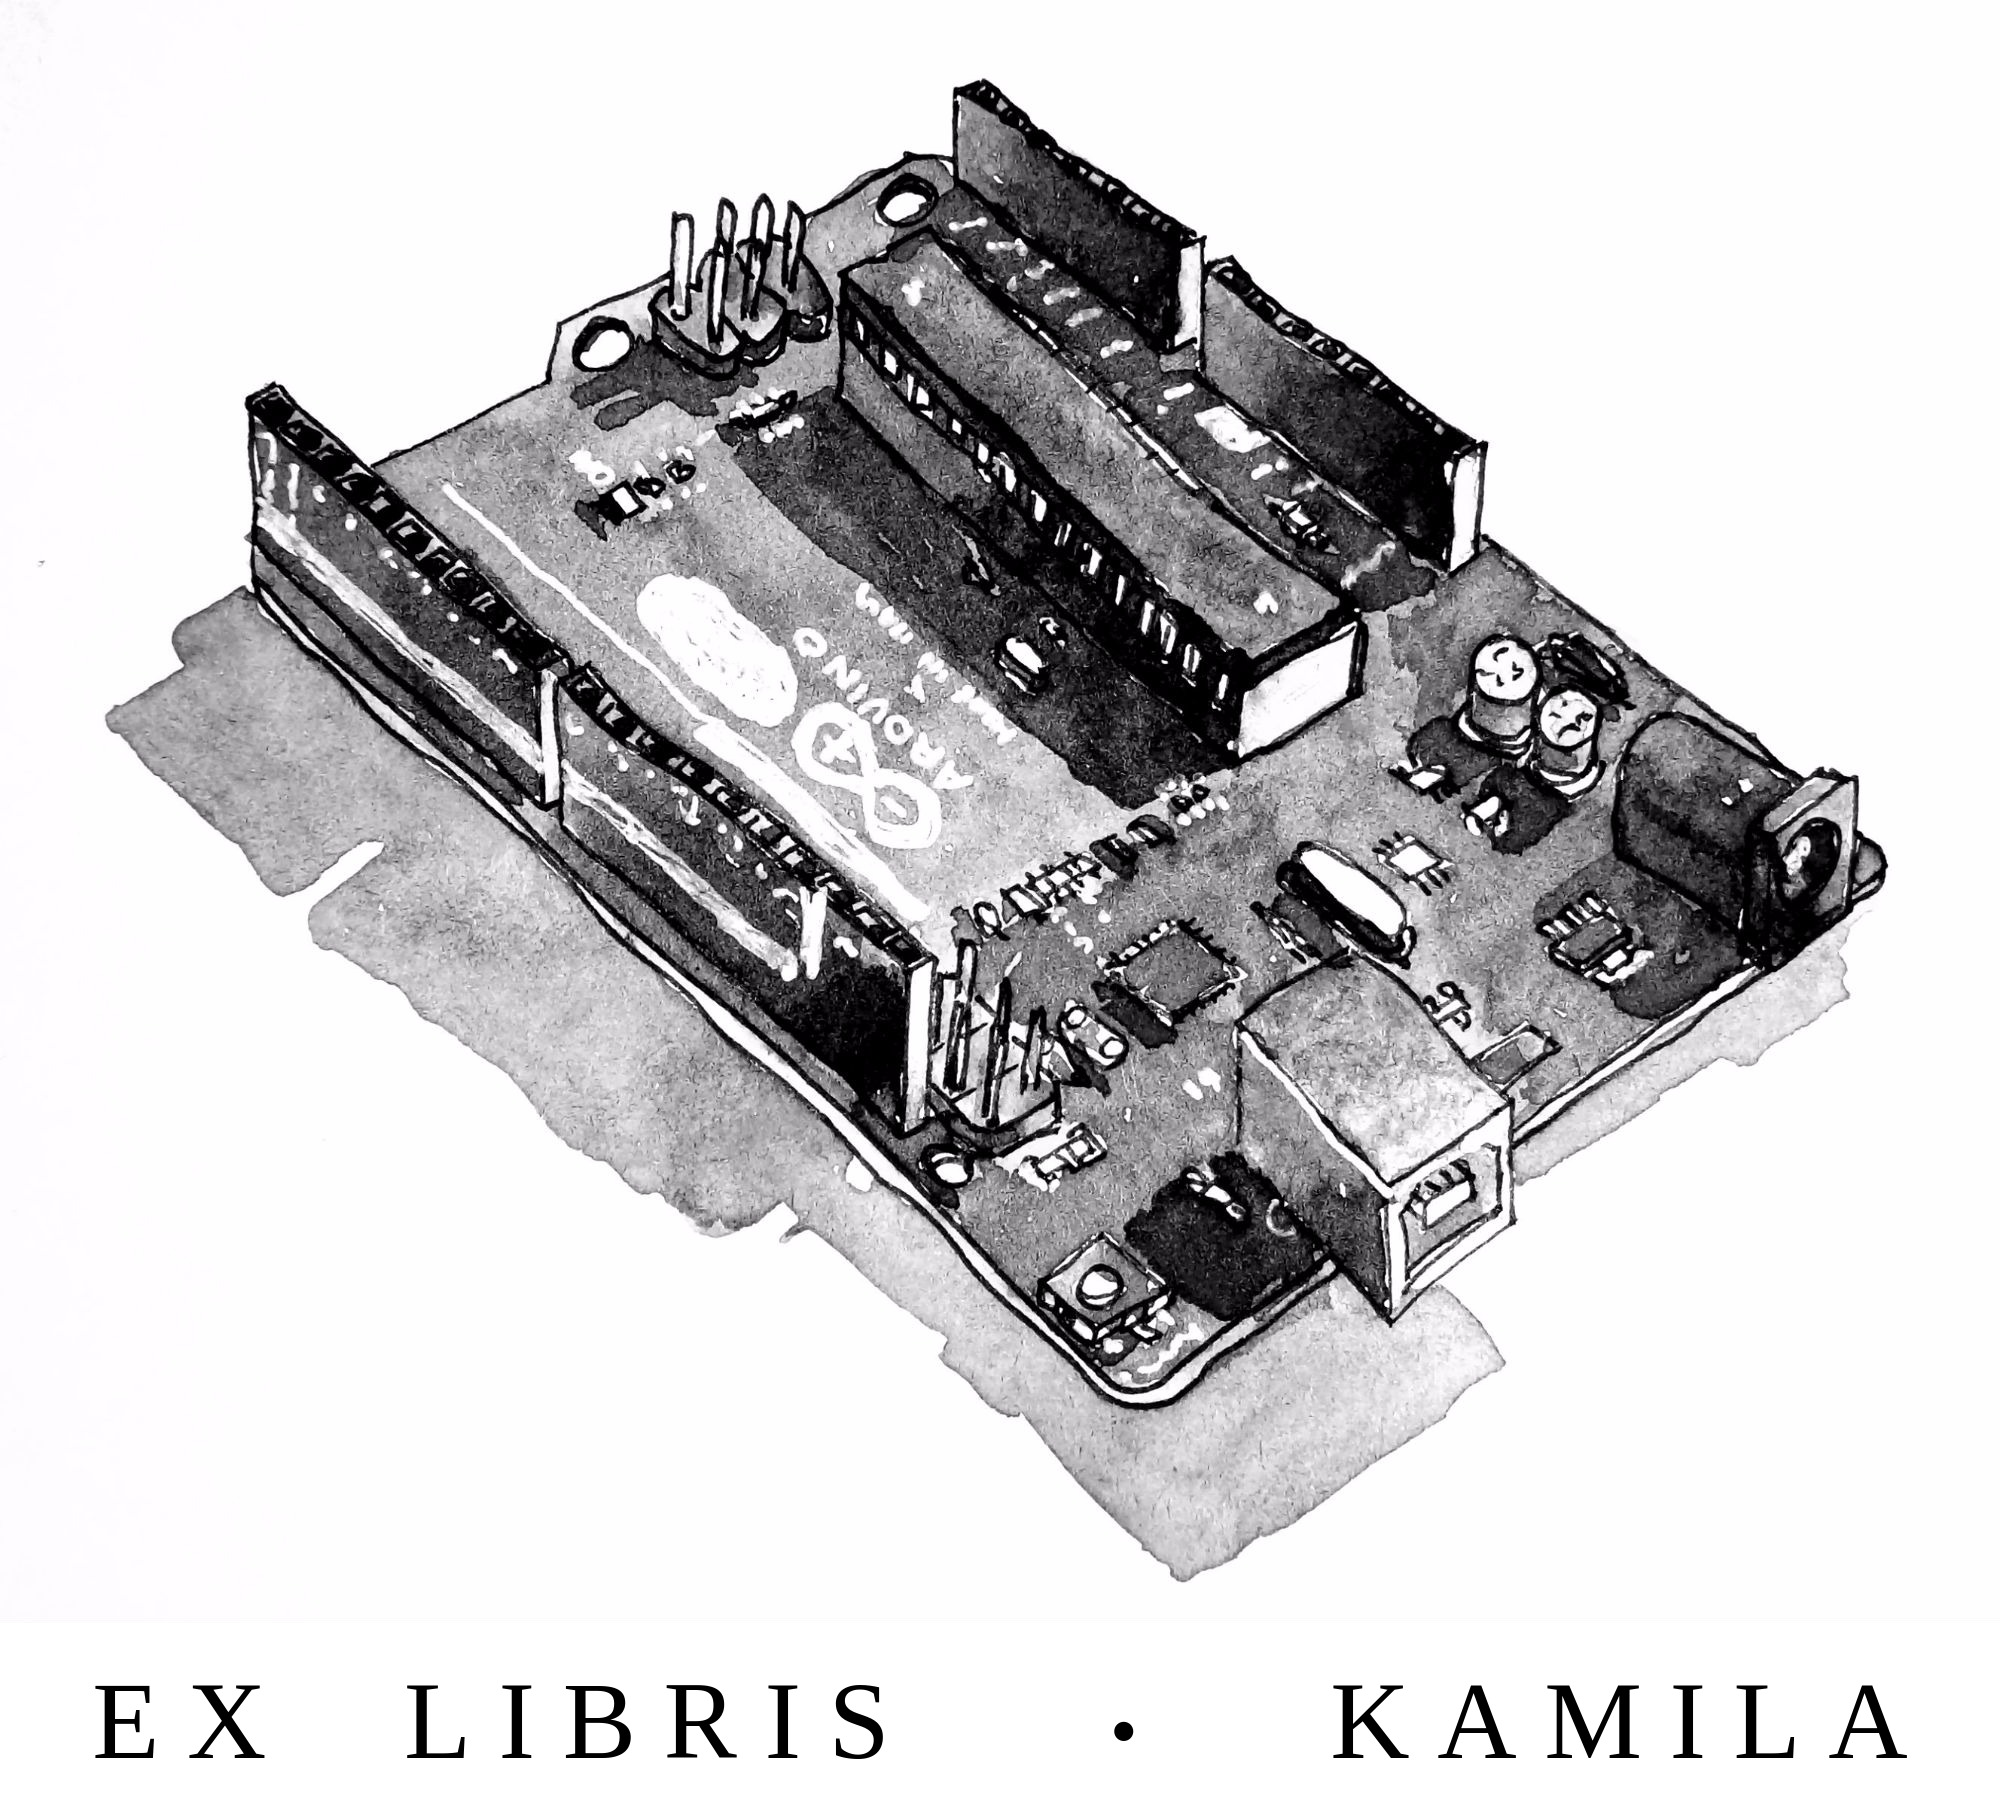
\includegraphics[width = 70mm]{arduino_dwg.jpg}

\vspace*{2cm}

Copyright \textcopyright \, Kamila Zdybał, 2017

For more documents similar to this one 

visit me on GitHub: @camillejr

To contact me personally drop me a line at:

\verb|kamilazdybal@gmail.com|

\end{center}
\newpage

% EX_LIBRIS_PAGE_TEMPLATE END ================================

\setlength{\parindent}{0cm}

\clearpage


\tableofcontents



\setlength{\parskip}{1em}
\renewcommand{\baselinestretch}{1.0}


\newpage


\chapter{Introduction} \label{chap:intro}

In October 2017 I have decided that I will be studying boundary layers for minimum 25 minutes every day. This document is a log of my journey that is still in progress. It's in the form of the notes and the record of my thoughts on the matters I studied.


\section{Mission objectives} \label{chap:objectives}

When you decide to sacrifice time and effort to pursue certain field of interest you'd better find very strong and realistic reasons for why you do that. Of course, it also has to bring you everyday pleasure, but in the times when it stops being a pleasure (and those times will come), you have to have something more to motivate you. At those times, when you're tired and don't feel like studying and you know that your brain won't absorb enough knowledge and that reading a textbook will be a nightmare, there are your reasons why you wanted to do that in the first place. They are your babies screaming at night and you just have to get up and feed them.

These are my reasons for why I study boundary layers:

\begin{enumerate}

\item I want to gain maths knowledge used in fluid dynamics, so that next subjects will be of less struggle in understanding calculus and become really the struggle to understand fluid dynamics concepts.

\item I want to understand Navier-Stokes equations. I want to gain intuitive feel for them and become comfortable about what every term means. I want to see their full power and see what their limitations are.

\item I want to build a knowledge toolbox to create Matlab / Python codes to simulate boundary layers phenomena.

\item I want to write this PDF that will contain a bunch of my-way-explanations of "difficult" concepts which will hopefully one day become a guide (that I always needed to find) for someone.

\item I want to become better at fluid dynamics in general so that even when there are amazing places like the von Karman Institute which can't take me for their programs because the government of my country didn't support their research, there might still be people who would like to help. I want to: "be so good that they can't ignore you".

\item This is something that I feel passionate about and I want to keep doing it regardless of any obstacles.

\item I want to do it my way.

\item I want to find among my journey enough knowledge and hope for building my own wind tunnel for studying boundary layers.

\end{enumerate}



\section{How to make it interesting} \label{chap:interesting}

This is a list of things that bring the pleasure to my studies:



\begin{enumerate}

\item Imagining how what I've learned could be used.

\item Imagining, and sometimes performing the experiments to verify what was said in the book.

\item Making thought experiments, sometimes imagining "what-if-worlds" that do not exist.

\item Imagining and writing Matlab / Python codes to simulate phenomena given in the textbook.

\item Doing things my way and doing things new way. 

\item Finding new ways to make things more interesting.

\item Explaining things on a white board / card board as if I was presenting it to someone.

\item Preparing an illustrative drawing to explain what was said in the book. Even if it's something that I've already understood.

\item Writing LaTeX documents.

\item Talking with friends about the things that I have learned. 

\end{enumerate}



\section{The learning curve} \label{chap:learning_curve}

\begin{figure}[H]
\centering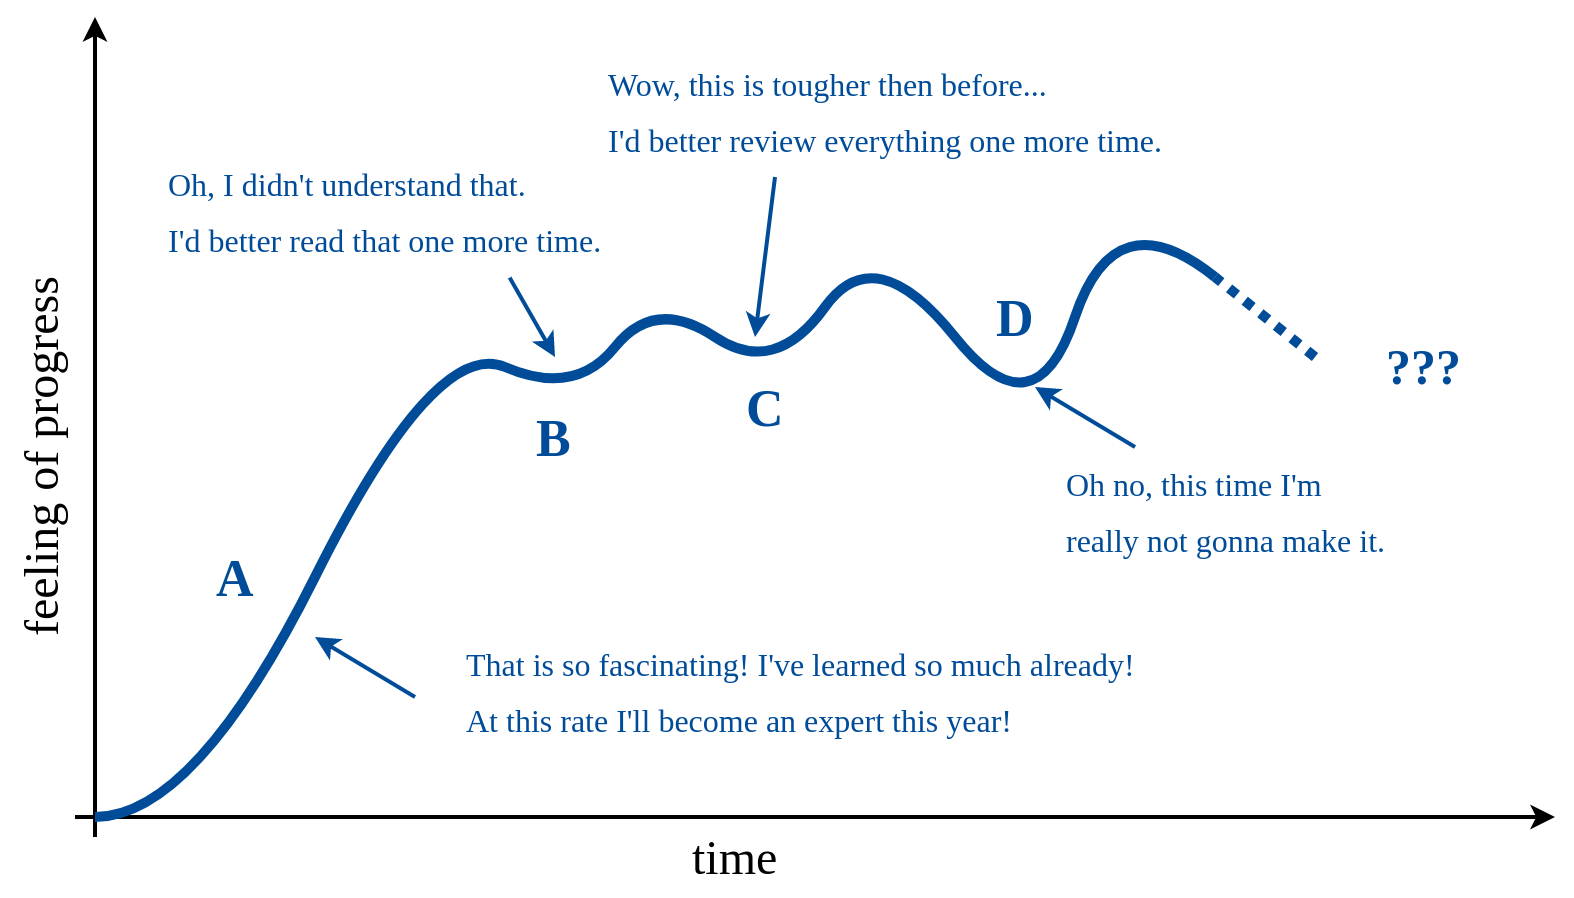
\includegraphics[width=14.5cm]{learning_curve}
\caption{The learning curve.}			
\label{fig:learning_curve}
\end{figure}


The difference is that if you aren't engaged with the subject you're very likely to quit. Either it's at D, earlier or later. I made a decision not to quit (and my reasons for why I started in the first place help me on the way). 


\section{The learning observations} \label{chap:learning_observations}


\section{How it's done}

I use the Pomodoro technique while I study. I use the app called Brain Focus and I typically set one Pomodoro of boundary layers studying per day. For these 25 minutes I try to be as focused solely on boundary layers as I can be.

Most often, I study before going to sleep because this allows me to turn off the computer screen and prepare myself for sleep by simply reading a paper book. Although sometimes this has a reverse effect on my sleep preparation when the section I'm reading gets really exciting.

\section{How does it look like}

I'm not always super happy about having to study boundary layers. Sometimes it gets late because I was busy with other things and I still have my 25 minutes of reading to do. There are days when I don't and go to bed. There are days when I force myself to read but I feel that I haven't learn anything useful. There are days when I force myself and after 5 minutes I realize that I have just came across an amazing thought and after my 25 minutes pass on Pomodoro I turn off the app and keep going. 

In other words, it's just like anything. I don't feel excited all the time. And I don't feel tired all the time. Statistically, the more you study the more days of excitement happen. And fortunately, they are the ones we remember and cherish the best.





\section{Sources of knowledge}


\textbf{EdX course - MITx: 16.110x 2 Flight Vehicle Aerodynamics} by Mark Drela










\chapter{Preliminaries}

This chapter is a record of what my "first 20 hours" looked like.


\section{World without friction} \label{chap:without_friction}

Imagine the world without friction.

Now imagine, that you move the palms of your hands against each other.

Do you feel the "shear" or "drag" on your hands?

- No. With no friction this is not present.

Do you feel the "pressing" of each palm on the other?

- Yes! I can feel it!

Perfect! There is no reason why you shouldn't. The forces perpendicular to your palms get transported from one to the other just fine.\footnote{Interesting distraction: can you think of a way to build a "frictionless world simulator", one that will allow you to feel the push on your hands when they get in close contact but at the same time you will not experience the shear when sliding your hands?}

Now, the same thing happens when we make an assumption that the fluid is perfect, ergo frictionless. Any object that such fluid will flow around will not experience the shear stress (or the drag). It will however experience the pressure force perpendicular to its outline.

There is a big consequence that comes from the above "monologue": if you want to study the drag on a body immersed in a fluid, you have to look at the world of friction.

That's why it's the high time to leave the frictionless considerations. It's of not much use in the subject of boundary layers - or the science of what happens at the very edge between the fluid and the solid body. Get ready for an awesome ride in the world of friction.



\chapter{The journey}


This chapter is a record of my journey. It is constantly in progress...

\section{Understanding the substantial derivative} \label{chap:deriv}

The substantial derivative is damn important. I've already had a chance to find about this in my previous pursuits of fluid mechanics. I remember it has been a challenge to really understand what the substantial derivative means and when I began my studying of BLs I realized that I either already forgot what I've once learned or I've never really understand it.

But this time I need to understand it deeply! So let's find a way to do that.

Imagine that you're walking on the streets of London with a bag of muffins. Every once in a while you reach to the bag to pick another muffin that you then endeavour because you're really a big fan of pastry and because the day is enjoyable and you want to feel happy.

On the street that you're currently strolling on there's a really good bakery and the croissants look so delicious from the shop window that you just have to walk inside to buy a few.

Then you take your bag of goodies and walk into the Buckingham Palace Gardens to eat the hell out of it. By the end of your walk you've finished the whole bag.

Now you take a seat on the park bench and in the warm sunlight you begin to wonder:

...if I were to analyse the change in time of the amount of pastry products inside my bag... what would it be...? Well, some change was due to me constantly eating the pastry through my whole journey. But there was also an increase in pastry when I bought the croissants. If I wasn't walking near that awesome bakery, there wouldn't be, so some change had to be dependent of where I was walking. Maybe if I chose my paths recklessly I might have even lost a few muffins to the outside world! Let me call the change of pastry in time by the term:

$\frac{Dp}{Dt}$

$p$ - standing for pastry

Then I'm going to call the continuous change due to eating (and independent of my path) the Local Change of $p$ ($LC_p$). And there has to be the term which is dependent of where I went which I'm going to call the Advective Change of $p$ ($AC_p$).

So the total change of pastry in time is simply the sum of the two:

\begin{equation}
\frac{Dp}{Dt} = LC_p + AC_p
\end{equation}






\section{Understanding the continuity equation}

Now when you see this in a textbook:

\begin{equation}
\frac{D \rho}{D t} = - \rho \text{div} \vec{\upsilon}
\end{equation}

it doesn't look so scary anymore! Even though we still don't \textbf{really} know what it means. But at least we have a feel for it.







So they claim that that is equivalent to this:

\begin{equation}
\frac{\partial \rho}{\partial t} = - \text{div} (\rho \vec{\upsilon})
\end{equation}

but why???

Let's see, in the 3-D case we have:

\begin{equation}
\frac{\partial \rho}{\partial t} = - \frac{\partial}{\partial x} (\rho \vec{\upsilon}) - \frac{\partial}{\partial y} (\rho \vec{\upsilon}) - \frac{\partial}{\partial z} (\rho \vec{\upsilon})
\end{equation}

In the most general case $\rho$ is a function of time and space. In 3-D it can be written as $\rho(t, x, y, z)$, so we have to apply the product rule to calculate the derivative of each term:

\begin{equation}
\frac{\partial \rho}{\partial t} = - \frac{\partial \rho}{\partial x} \vec{\upsilon} - \frac{\partial \vec{\upsilon}}{\partial x} \rho - \frac{\partial \rho}{\partial y} \vec{\upsilon} - \frac{\partial \vec{\upsilon}}{\partial y} \rho - \frac{\partial \rho}{\partial z} \vec{\upsilon} - \frac{\partial \vec{\upsilon}}{\partial z} \rho 
\end{equation}

\begin{equation}
\frac{\partial \rho}{\partial t} + \frac{\partial \rho}{\partial x} \vec{\upsilon} + \frac{\partial \rho}{\partial y} \vec{\upsilon} + \frac{\partial \rho}{\partial z} \vec{\upsilon} =  - \frac{\partial \vec{\upsilon}}{\partial x} \rho - \frac{\partial \vec{\upsilon}}{\partial y} \rho - \frac{\partial \vec{\upsilon}}{\partial z} \rho
\end{equation}

By definition of the partial derivative:

\begin{equation}
\frac{\partial \rho}{\partial t} + \frac{\partial \rho}{\partial x} \vec{\upsilon} + \frac{\partial \rho}{\partial y} \vec{\upsilon} + \frac{\partial \rho}{\partial z} \vec{\upsilon} = \frac{D \rho}{D t}
\end{equation}

and by observing that the right hand sides is much like the divergence of something:

\begin{equation}
- \frac{\partial \vec{\upsilon}}{\partial x} \rho - \frac{\partial \vec{\upsilon}}{\partial y} \rho - \frac{\partial \vec{\upsilon}}{\partial z} \rho = - \rho \text{div} \vec{\upsilon}
\end{equation}

voila:

\begin{equation}
\frac{D \rho}{D t} = - \rho \text{div} \vec{\upsilon}
\end{equation}

\section{Making use of $F = ma$} \label{chap:momentum}

A close companion of the continuity equation is the momentum equation. I bet you'll meet them in a close proximity when you read any fluid textbook. Some authors simply write them out thinking that people will learn through exposure\footnote{\textit{Learning through exposure} (n.) - a process of learning something just by being around it for a significant amount of time.}. And you begin to feel stupid that you didn't understand them by looking at them.

One breakthrough in the study of the momentum equations was when I realized that it was just "$F=ma$"\footnote{Yay for Newton.}. But a more fancy one. Let me prove that for you:

\begin{equation}
\rho \frac{D \vec{\upsilon}}{Dt} = \vec{f} + \vec{P}
\label{eq:momentum}
\end{equation}

In fact, the way I wrote this here is more of "$ma=F$". On the right hand side you have the net force acting on a fluid volume - there's the friction force $\vec{f}$ and the pressure force $\vec{P}$ - the only two taken into account. On the left hand side you have mass times acceleration, with acceleration being $\frac{D \vec{\upsilon}}{Dt}$. You might ask now: what mass? I don't see any! 

Well, yeah. The equation \ref{eq:momentum} is given \textbf{per unit volume}. And so the truth is that it's more of a "$\frac{F}{dV} = \frac{ma}{dV}$". 

By the way, if you've ever wondered what $dV$ looks like, here it is:

\begin{figure}[H]
\centering\includegraphics[width=10cm]{dV}
\caption{Model of the infinitesimal volume, scale $\infty$:1.}			
\label{fig:infinitesimals}
\end{figure}


When you divide mass per volume you get density. But it also means that the terms on the right hand side cannot have the unit of force but the force per volume as well. $\vec{f}$ is in fact friction force per unit volume and $\vec{P}$ is pressure force per unit volume.



So if they simply describe the sum of forces why are they called "momentum" equations and not, for example, the "force" equations?



\section{The role of viscosity inside the boundary layer} \label{chap:viscosity}











\chapter{The questions}

This is a collection of questions that I have during my studying. I want to keep track of the things that I didn't understand and want to understand.

\begin{enumerate}
\item Why is nondimensional so sexy?
\end{enumerate}


\newpage

\begin{thebibliography}{50}



\end{thebibliography}

\end{document}
